%!TEX root = mainfile.tex

\section{The Hubble Space Telescope} % (fold)
\label{sec:the_hubble_space_telescope}

	\subsection{Mission Launch} % (fold)
	\label{ssub:mission_launch}
		On April 24th 1990 NASA’s Space Shuttle Discovery launched the world’s first space-based optical telescope; The Hubble Space Telescope (HST), named in honour of American astronomer Edwin P. Hubble. Edwin Hubble’s greatest contribution to astronomy was the Hubble Law which states that galaxies are receding from us at a speed directly proportional to their distance from us. This showed that our universe is expanding, a notion which underpins modern cosmological thinking. The telescope sits in a low-Earth orbit, as shown in figure~\ref{fig:hubble_space_telescope}, at an altitude of 569 kilometres completing one orbit of the Earth every 97\,minutes\cite{Hubsite_1}.
		\begin{figure}[ht]
			\centering
			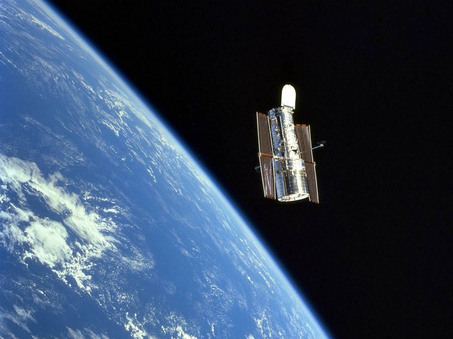
\includegraphics[width=0.5\textwidth]{../Images/Hubble_Space_Telescope.jpg}
			\caption{Photograph of HST orbiting the Earth.\label{fig:hubble_space_telescope}}
		\end{figure}

		The HST was designed to provide clear and deep views of distant galaxies and stars and most of the planets in our solar system. Hubble's domain extends from the ultraviolet through the visible and into the near-infrared\cite{NASA_1}.
	% subsection mission_launch (end)

	\subsection{Achievements to Date} % (fold)
	\label{ssub:achievements_to_date}
		The HST has provided unprecedented detail in images of star formation allowing astronomers to see the jets and disks present during the birth of new stars. It has also been able to study the atmospheric composition of extra-solar planets and take the first visible light picture of a planet outside our solar system; Fomalhaut b\cite{Hubsite_3}.

		Many EoR galaxies and candidate galaxies have been identified using HST data. In December 1995 the HST was pointed at what was believed to be a fairly empty and uninteresting patch of sky; 342 separate exposures were taken over 10 consecutive days and formed an image called the Hubble Deep Field (HDF)\cite{ESA_2}. The image contains around 3,000 objects of which the vast majority are galaxies, with a few local stars in the foreground. The HDF is one of the most iconic images of the 20th century, and it has since been cited in over 800 scientific papers.

		In 2004 its successor was revealed, the Hubble Ultra Deep Field (UDF); a million-second exposure in a 200\si{\arcsecond}$\times$200\si{\arcsecond} area of sky containing \num{10000} galaxies stretching back 13\,billion years\cite{Hubsite_2}. This exposure utilised the recently installed Advanced Camera for Surveys (ACS), seen in figure~\ref{fig:HUDF}. This survey was further refined in September 2012 in the Hubble eXtreme Deep Field (XDF) which utilised the recently installed WFC3 camera as well as combining over \num{2000} separate exposures from different sources\cite{ESA_2}.
		\begin{figure}[ht]
			\centering
			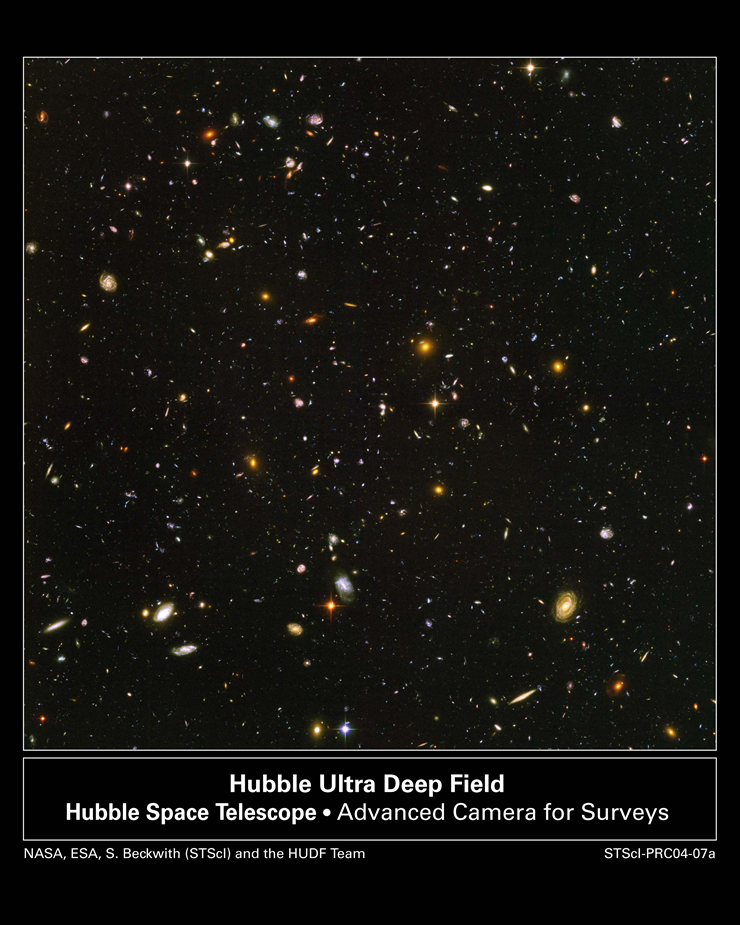
\includegraphics[width=0.8\textwidth]{../Images/HUDF.png}
			\caption{The HUbble Ultra Deep Field.\label{fig:HUDF}}
		\end{figure}

		Using data from the HUDF, object UDFj-39546284 was identified. In a paper by Bouwens et al, published in 2012, their best fit places it at a redshift of $11.8\pm0.3$\cite{Bouwens2012}. This would classify it as the oldest object ever observed. The exact nature of the object is not known but it is believed to be a mini-galaxy. Confirmation will require spectroscopic analysis, which is likely to be carried out by the James Webb Space Telescope. This observation demonstrates both the achievements and limits of the current technology.
	% subsection achievements_to_date (end)

	\subsection{Operation} % (fold)
	\label{ssub:operation}
		The HST is operated remotely from the earth, it has 4 antennae which can send and receive signals from the Flight Operations Team at Goddard Space Flight Centre in Greenbelt, Maryland via the Tracking and Data Relay Satellite system. For communication to be possible HST must have a direct line of sight to at least one of these 5 satellites.

		The HST is powered using 2 arrays of solar panels each capable of converting the Sun’s rays into \num{2800} watts of electricity. The arrays are able to store the electricity in batteries allowing the HST to remain active while in the Earth’s shadow (approximately 36\,minutes out of every 97\,minute orbit).

		Orbiting the Earth subjects the HST to extreme conditions due to the effect of zero gravity and the variation in temperature (up to around \SI{40}{\kelvin}) during each orbit. The optical system is held together using a skeleton (truss) constructed from Graphite epoxy. Graphite epoxy, commonly found in racquets and golf clubs is a stiff and lightweight material able to resist expansion and contraction due to temperature changes\cite{Hubsite_4}.
	% subsection operation (end)

	\subsection{Performance and Optical Telescope Array} % (fold)
	\label{ssub:performance_and_optical_telescope_array}
		The HST is constructed using a Ritchey-Chretien Cassegrain design; this allows high-performance over a wide field of view. The incoming light enters a tube with baffles removing any unwanted stray light, as shown in figure~\ref{fig:HST_optical_diagram} below. The light is then collected by the concave Primary mirror and reflected towards the smaller convex Secondary mirror. This light is then reflected back through a hole in the centre of the Primary mirror where it is focused onto a small area to be picked up by the instruments\cite{Hubsite_5}.
		\begin{figure}[ht]
			\centering
			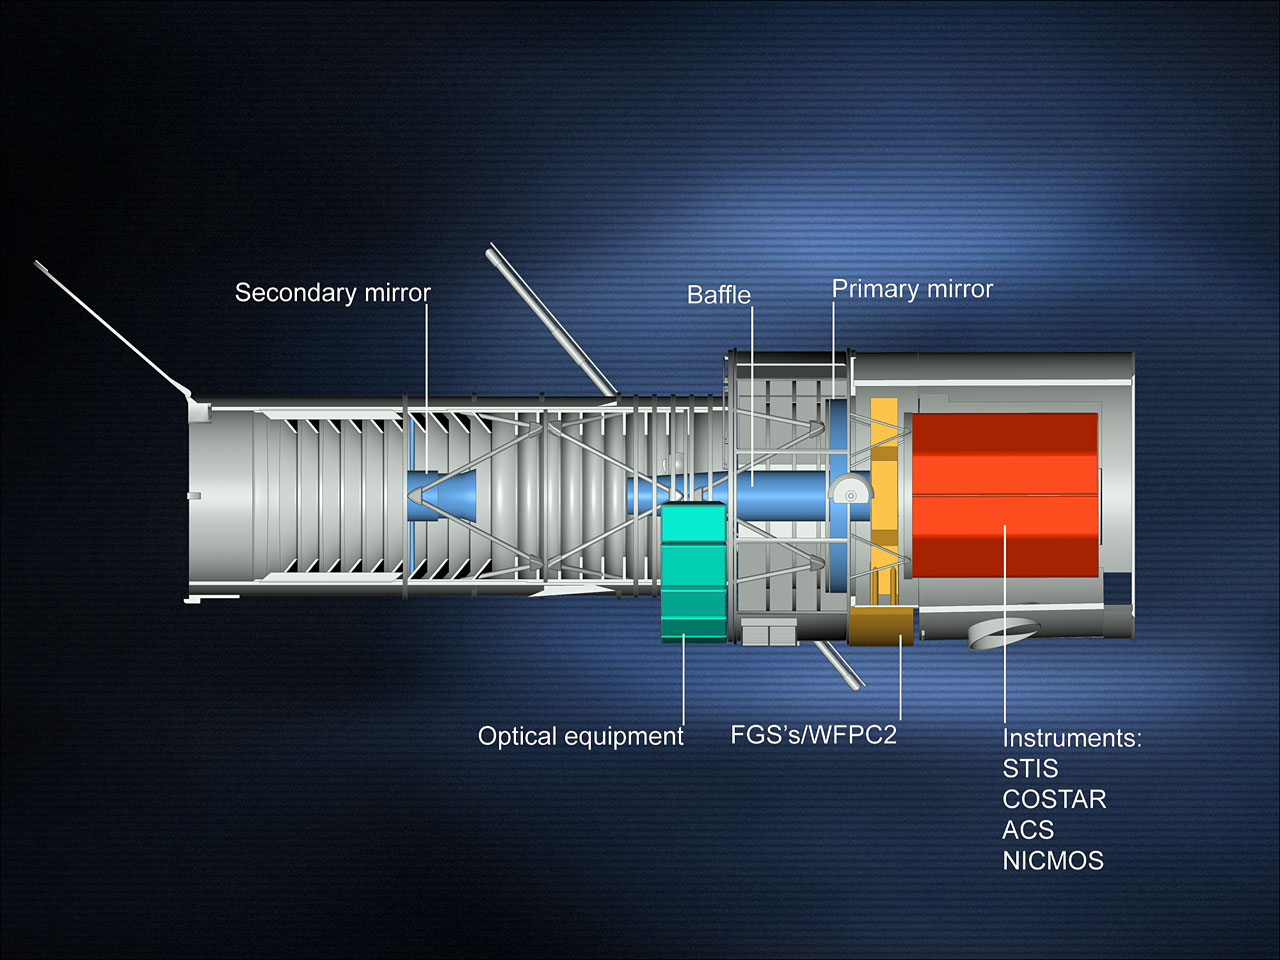
\includegraphics[width=0.5\textwidth]{../Images/HST_optical_diagram.jpg}
			\caption{Diagram showing basic systems of HST, note that WFC2 has since been replaced by WFC3.\label{fig:HST_optical_diagram}}
		\end{figure}

		The mirrors have been polished to an accuracy of better than the wavelength of visible light. When the HST was first launched the scientists soon realised that the curve to which the mirrors had been ground was not correct resulting in an error known as spherical aberration which blurred the images. A servicing mission in December 1993 deployed 5 pairs of mirrors which were able to successfully correct the error and allow Hubble to take the images it was intended to\cite{ESA_1}.

		There have been 4 servicing missions sent to the HST with the final mission taking place in May 2009. Over its lifetime the cameras and instruments have undergone many improvements and replacements. The camera currently operating that is of interest to this project is the WFC3/IR camera, installed in 2009. This camera is able to observe in the near-infra-red where we expect to see the Lyman-break galaxies. Table~\ref{tab:HST_technical} shows the key technical data for the HST, amazingly the HST is so precise it is able to lock onto a target at a distance of 1 mile without deviating more than the width of a human hair.
		\begin{table}[ht]
			\begin{center}
				\begin{tabular}{l|l}
					Component	& 	Details \\
					\hline\hline
					Primary Mirror Diameter & \SI{2.4}{\metre} \\ \hline
					Secondary Mirror Diameter & \SI{0.3}{\metre} \\ \hline
					Wavelength range & 800--1700\si{\nano\metre} \\ \hline
					Total Field of View & \SI{123}{\arcsecond}$\times$\SI{136}{\arcsecond} (\SI{16728}{\arcsecond}$^2$) \\ \hline
					Pixel Size & $18\times18$\,\si{\micro\metre} \\ \hline
					Plate Scale & \SI{0.13}{\arcsecond\per\pixel} \\ \hline
					\multirow{3}{*}{Quantum Efficiency} & 77\% at \SI{1000}{\nano\metre}\\
					 & 79\% at \SI{1400}{\nano\metre}\\
					 & 79\% at \SI{1650}{\nano\metre}\\ \hline
					Dark count &  \SI{0.048}{\electron\per\second\per\pixel} \\ \hline
					Readout noise & \SI{12.0}{\electron\per\second\per\pixel} \\ \hline
					Full Well & \SI{77900}{\electron} \\ \hline
					Gain & 2.28--2.47\si{\electron\per\ADU} \\ \hline
					Operating Temperature & \SI{145}{\kelvin} \\ \hline
					FWHM & \SI{0.151}{\arcminute} at \SI{1600}{\nano\metre}
				\end{tabular}
			\end{center}
			\caption{Technical data for HST WFC3/IR camera system\cite{WFC3_IHB}}
		\label{tab:HST_technical}
		\end{table}
	% subsection performance_and_optical_telescope_array (end)

% section the_hubble_space_telescope (end)
